\documentclass[conference]{IEEEtran}
\usepackage{graphicx}
\usepackage{latexsym}
\usepackage{enumerate}
%\usepackage{ascmac}
\usepackage{url}
%\usepackage{fancybox}
%\usepackage{subfigure}
\usepackage{mediabb}
%\usepackage{color}

\graphicspath{{./figures/}}
\newcommand{\figref}[1]{Figure \ref{#1}}
\newcommand{\tabref}[1]{Table \ref{#1}}
\newcommand{\secref}[1]{Section \ref{#1}}

\hyphenation{op-tical net-works semi-conduc-tor}

\begin{document}

\title{ROCAT on KATARIBE:\\ Code Visualization for Communities}

\author{
\IEEEauthorblockN{
Tomohiro Ichinose\IEEEauthorrefmark{1},
Kyohei Uemura\IEEEauthorrefmark{1},
Daiki Tanaka\IEEEauthorrefmark{1},
Hideaki Hata\IEEEauthorrefmark{1},
Hajimu Iida\IEEEauthorrefmark{1},
Kenichi Matsumoto\IEEEauthorrefmark{1}
}

%\IEEEauthorblockN{
%Yusuke Saito\IEEEauthorrefmark{1},
%Shin Fujiwara\IEEEauthorrefmark{1},
%Kenji Fujiwara\IEEEauthorrefmark{1},
%Stevche Radevski\IEEEauthorrefmark{1},\\
%Hideaki Hata\IEEEauthorrefmark{1},
%Hajimu Iida\IEEEauthorrefmark{1},
%Kenichi Matsumoto\IEEEauthorrefmark{1}
%}
\IEEEauthorblockA{\IEEEauthorrefmark{1}Graduate School of Information Science,
Nara Institute of Science and Technology\\
Takayama 8916-5, Ikoma, Nara,
630-0192 Japan\\
Email: \{ichinose.tomohiro.ik1@is, uemura.kyohei.ub9@is, tanaka.daiki.sx4@is, hata@is, iida@itc, matumoto@is\}.naist.jp}
}
%Email: \{saito.yusuke.sl9, fujiwara.shin.fe5, kenji-f, stevche.radevski.sl1, hata\}@is.naist.jp,\\
%iida@itc.naist.jp, matumoto@is.naist.jp}
%}

\maketitle

\begin{abstract}
As globally distributed software development has become generalized, social coding platforms like Github are becoming increasing needed for team collaboration. 
To share and help understand the overview of projects among teams, source code visualization is useful. 
In this paper, we present a new visual software development tool, Rocat, a  city-like software code visualization in virtual reality.
In addition, we integrate Rocat with a GitLabbased code hosting service, Kataribe. By integrating Rocat into Kataribe, fine-grained code information can be visualized, and city visualization can be easily shared. 
We present our tool and provide the features of Rocat on Kataribe.
A Screencast for demonstration is available at the following URL.\\
\url{https://www.youtube.com/watch?v=ZQTTO91v4No}
\end{abstract}



\section{Introduction}
Since the beginning of software development, the size and complexity of software have been continuously on the rise.
If the software for a space shuttle 30 years ago was 400,000 lines of code, nowadays even a smartphone application can easily exceed that size.
Not only has the size of software increased in terms of LOC, but integration and interaction with external services has also dramatically increased.
However, with the increase in size and complexity, comprehending the structure and analytics of software, especially without a good way to visualize the information has become increasing difficult.

One good way to represent software structure, size, and modularity is \textsf{CodeCity} \cite{Wettel:2011:SSC:1985793.1985868}, which represents classes as buildings and packages as districts in 3D, similar to a city.
Since the original \textsf{CodeCity} does not offer a great number of interactions for a developer with a city, there has been some work to extend it. 
One interesting approach is \textsf{CodeMetropolis} \cite{6648194}, where software cities are represented in \textsf{Minecraft}, allowing for better collaboration within the \textsf{Minecraft} game.
Showing similar data as \textsf{CodeCity}, \textsf{CodeMetropolis} allows the user to walk around the city and interact closely with the buildings (this is the source code).
The same representation has also been used to specifically represent the development history of a city using a bird's-eye view \cite{Steinbruckner:2010:RDH:1879211.1879239}.
Each approach has its own purpose, but all approaches assist in the understanding of the software.

\begin{figure}[h]
\centering
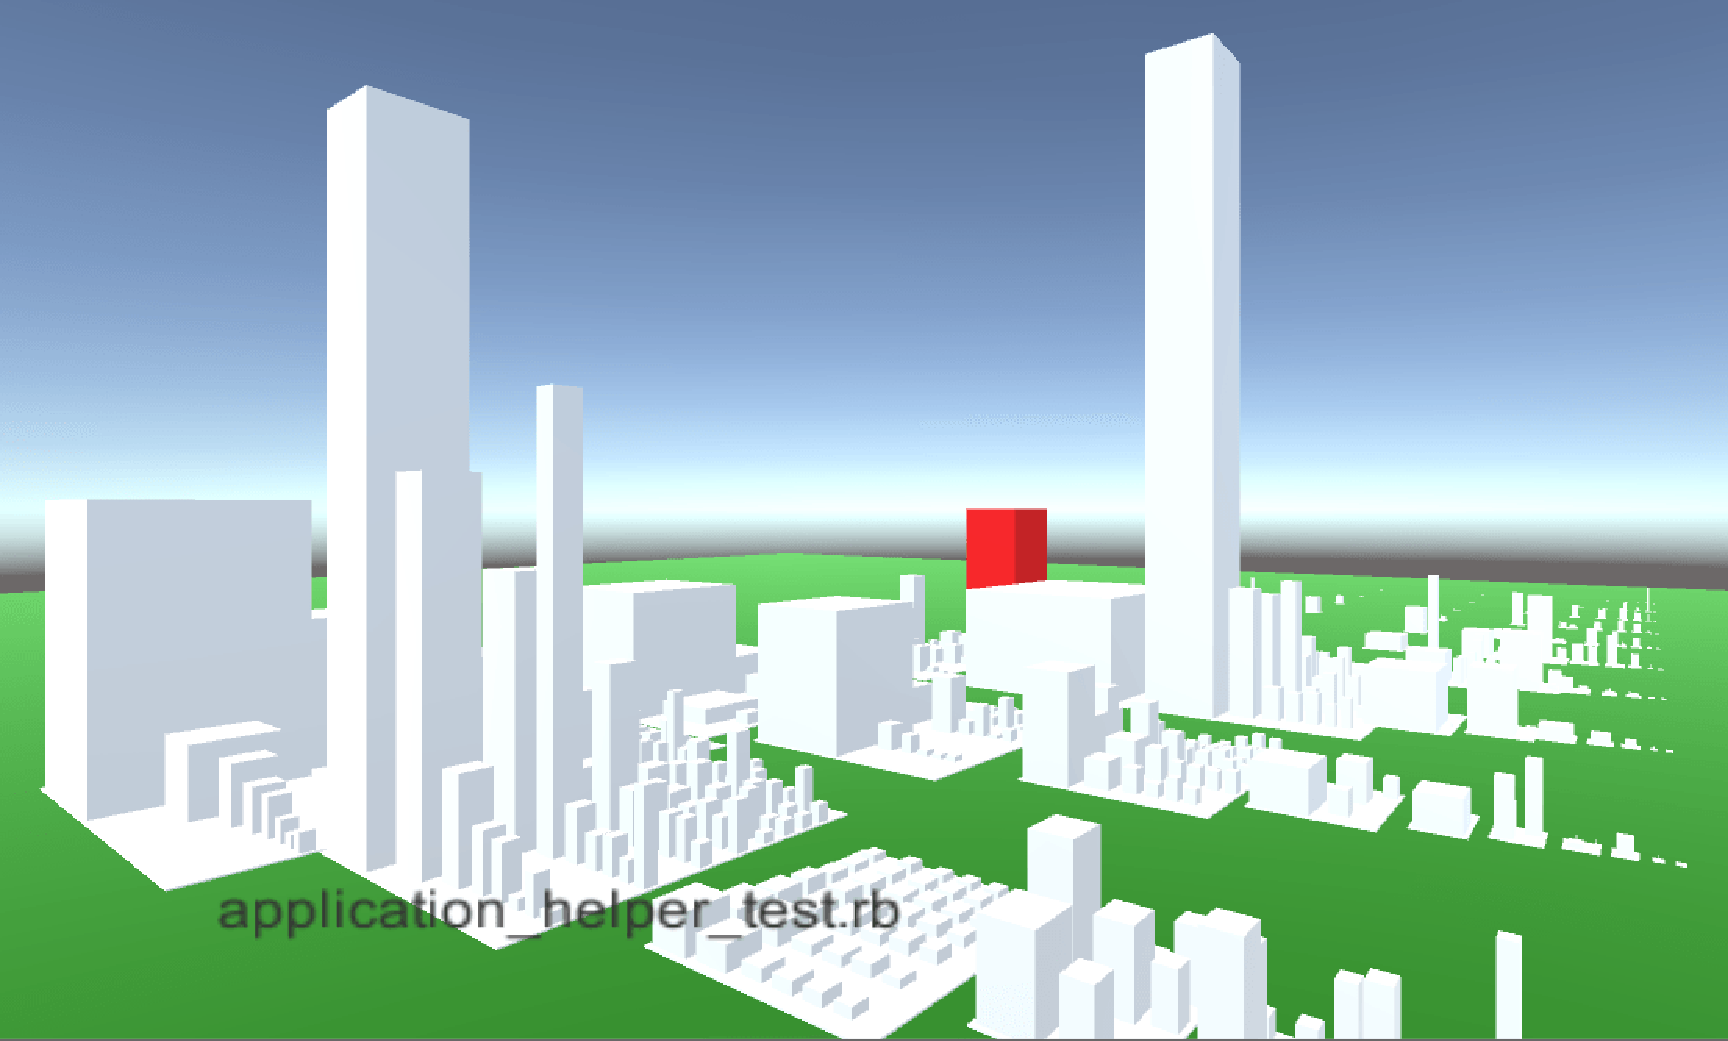
\includegraphics[width=8cm]{NewROCAT.pdf}
\caption{City-like code visualization}
\label{figure:new-Rocat}
\end{figure}

The reason we believe these visualization techniques are good is because of the ease in understanding the structure of the software, the class size, and the number of packages within seconds.
Furthermore, humans are very good at processing very large amounts of information in real-world city-like views quite quickly since we learn and adapt to the environments we live in.
For example, just by glancing at a building, it is usually possible to tell the age of the building, i.e., whether it has a modern or classic design, the material it is made of, the color, and more. 
That being said, using a visualization technique that is similar to the real-world allows us to map the meanings of characteristics from the real-world to some aspect of the software, processing it with a similar speed as we would process the meaning of the real-world object.

Even though we believe the previously mentioned approaches are useful for visualizing software, we think that the full potential of such visualization techniques have not been fully utilized.
These approaches use the concepts of a city to some extent, but they have not included many other aspects that real cities have and that can be used to deliver even more information to software engineers. 
If we manage to grasp this potential and use it in a way that is consistent with how we process information in a real environment, understanding the elements of a software system will get become faster and less superficial.

For this reason we want to extend the ways in which software cities can reflect real cities.
We want to provide an experience where the software engineer is immersed in the software, exploring and learning (maybe even subconsciously) about it while walking around, in the same way a person would explore a real city.
We would like to allow the engineer to naturally interact with the information and source code of the software so that such an enriched experience could help in better retention of information, as well as in easier comprehension.
To realize such system, we present a visualization tool, \textsf{Rocat}, which shows a city-like code visualization in a virtual reality environment.


\begin{figure*}[t!]
\centering
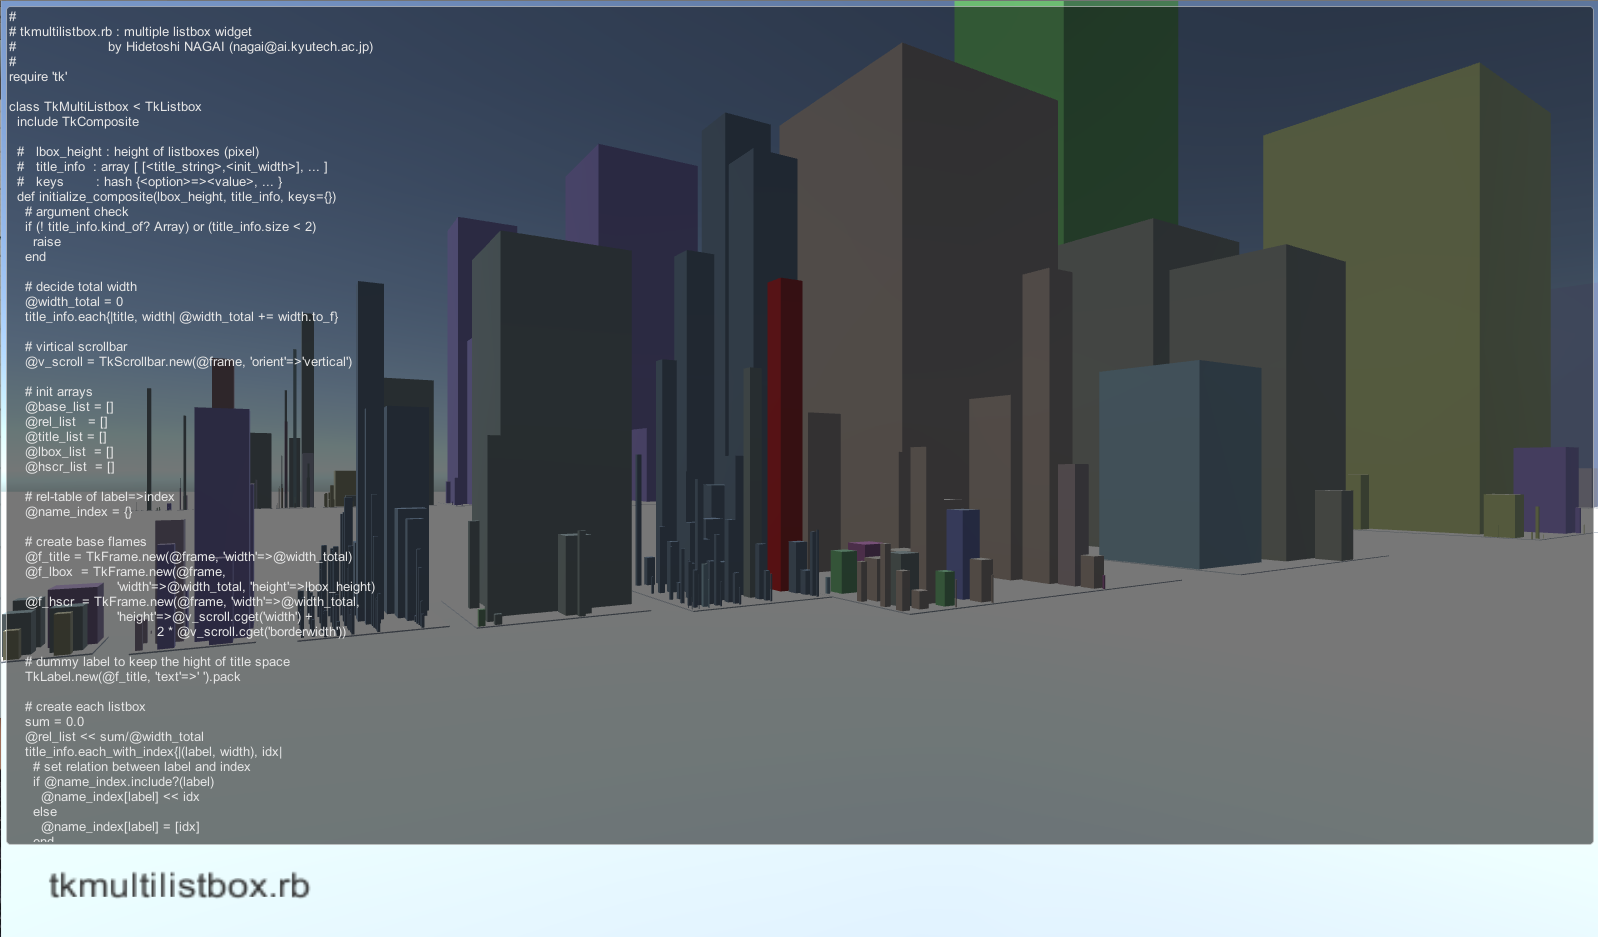
\includegraphics[bb=0 0 1598 937, width=18cm]{rocat.png}
\caption{Snapshot of \textsf{Rocat}}
\label{figure:Rocat}
\end{figure*}


In addition, we would like to introduce a new concept of code visualization, called \textit{code visualization for communities}.
Previous visualization tools focused mainly on supporting developers, a single developer \cite{Wettel:2011:SSC:1985793.1985868} or a team of developers \cite{6648194}.
However, we think that visualization should be beneficial for communities too since the effectiveness of social coding \cite{Dabbish:2012:SCG:2145204.2145396} and pull-based development \cite{Gousios:2014:ESP:2568225.2568260} has been made clear.
To address this challenge, we integrated the \textsf{Rocat} visualization system on \textsf{Kataribe},  our code hosting service.
With this kind of system, communities can share a large amount of information about the underlying software in a way that is quick and easy to understand.


\section{Rocat: Software Visualization}
To allow and support developers in comprehending source code and the conditions of projects, we propose \textsf{Rocat}, where developers can feel the code as if in an actual city, which will provide richer experiences for the developer by enabling exploration of the city. 
If the information represented about a building (or city) and its meaning is similar with a real-world city, it will be easy to quickly retrieve the meaning of what they view. 
In this section, we provide an overview and an implementation of \textsf{Rocat} for further usage.

\subsection{Overview and Implementation}
\textsf{Rocat} is a visualization tool that can be applied to multiple software development environments. 
\figref{figure:Rocat} illustrates a snapshot of a city-like view in  \textsf{Rocat}.
Similar to \textsf{CodeCity} \cite{Wettel:2011:SSC:1985793.1985868}, extracted metrics are mapped on the height and the base size of buildings.
The height represents the LOC and the base size represents the number of comments of the source code in the current system.
Users can explore the city among the buildings. 
When one building is selected (for example, the red building in the figure), its source code can be available on demand. 
It is possible to edit this source code with this view.
The color of the building describes the top contributor of the file corresponds to the building (the color of each contributor is selected randomly).
These colors can be used to find out which developer understands the software and is responsible for certain source code file.

Although \textsf{CodeMetropolis} is realized on top of an attractive popular role-playing game,  \textsf{Minecraft}\footnote{\url{https://minecraft.net/}} \cite{6648194}, we have started implementation using a cross-platform game engine, \textsf{Unity}\footnote{\url{https://unity3d.com/}}.
This is because we do not want to limit \textsf{Rocat} to specific purposes, but want to develop a general software development platform in the future. 
By using \textsf{Unity}, \textsf{Rocat} can be run on a web browser or any platform and can adopt \textsf{Oculus Rift} to using \textsf{Rocat} in virtual reality.

\textsf{Rocat} is not the only visualization possible, but it leads to a novel software development environment.
We describe our concept with the following related approach.

\begin{figure*}[tb]
\centering
\includegraphics[width=\linewidth]{Rocat-on-kataribe2.pdf}
\caption{Snapshot of \textsf{Rocat} on \textsf{Kataribe}}
\label{figure:Rocat-on-kataribe}
\end{figure*}


\subsection{Concept}
\subsubsection{Virtual Museum}
A virtual museum is a digital entity that draws on the characteristics of a museum in order to complement, enhance, or augment the museum experience through personalization, interactivity, and a richness of content\footnote{\url{https://en.wikipedia.org/wiki/Virtual_museum}}.
torytelling is one of the aims of virtual museums, which aim to make cultural content more attractive for the public and, consequently, the learning process easier \cite{Pietroni:2014:IVR:2635823.2611375}.
This aim is also important for \textsf{Rocat}.

\subsubsection{Web Maps}
Web maps like \textsf{Google Maps}\footnote{\url{https://maps.google.com/}} are indispensable for exploring real world cities.
Among various useful features, a zooming feature is one of the most basic and essential in comprehending the structure of cities. 
\textsf{Rocat} provides hierarchical views from a bird's-eye view to an explorative view.
From bird's-eye views, developers can glance at the characteristics of parts of projects or the entire project.
With explorative views, developers can investigate each building as well as the neighboring buildings.

\subsubsection{Visual Software Analytics Platform}
Software analytics is an analytics on software data for managers and software engineers with the aim of empowering individual and team software developers to gain and share insights from their data to make better decisions \cite{Menzies:2013:SAS:2553351.2553360} \textsf{SAMOA} is a visual software analytics platform \cite{6676936}.
Because \textsf{Rocat} is also a software development environment, it needs help in decision-making, that is, \textsf{Rocat} can be a visual software analytics system too.
\textsf{SAMOA} is a 2D system with different views: a snapshot view, an evolution view, and an ecosystem view.
Introducing these kinds of views in 3D environments should be helpful.

\subsubsection{Team Collaboration Platform}
From an empirical study of modern code review, Bacchelli and Bird report the motivations for code review \cite{Bacchelli:2013:EOC:2486788.2486882}. 
Although finding defects is still the main motivation, reviewers can also expect additional benefits such as knowledge transfer, increased team awareness, sharing code ownership, and so on. 
To support these outcomes, \textsf{Rocat} can also be helpful; that is, \textsf{Rocat} can be a team collaboration platform too.


\section{Kataribe: Fine-grained Code Hosting}
\textsf{Kataribe}\footnote{http://sdlab.naist.jp/kataribe/} is a hosting service of \textsf{Historage} repositories \cite{Fujiwara:2014:KHS:2597073.2597125}.
\textsf{Historage} repositories are fine-grained source code repositories \cite{Hata:2011:HFV:2024445.2024463}, and are converted from file-level Git repositories with a tool, \textsf{Kenja}\footnote{\url{http://github.com/niyaton/kenja}}.
\textsf{Kenja} constructs a directory structure for the \textsf{Historage} based on the result of syntactic analysis of all source code files in each commit.
Currently, \textsf{Kataribe} hosts \textsf{Historage} written in C\#, Go, Python and Ruby, since \textsf{Kenja} can only construct on those programming languages.
\textsf{Kataribe} uses \textsf{Gitlab}, which is a well-known OSS for hosting Git repositories.
Users can get \textsf{Historage} repositories from \textsf{Kataribe} without registration.
Registration at \textsf{Kataribe} enables users to browse \textsf{Historage} repositories on the Web.
\textsf{Gitlab} enables users to see logs and graphical statics of repositories.

Features of \textsf{Kataribe} include importing existing Git repositories that are provided on Git hosting services such as \textsf{Github} and also constructing \textsf{Historage} repositories incrementally.
Since a \textsf{Historage} repository created by \textsf{Kenja} is separated from the original repositories, users of \textsf{Kataribe} can continue their development regardless of their \textsf{Historage} repositories.
When a developer pushes her/his commits into their original repositories, \textsf{Kataribe} automatically converts pushed commits into the corresponding \textsf{Historage} repositories.
These features allow researchers to get the latest fine-grained histories when they want to start their new research.


\section{Rocat on Kataribe}
We integrate \textsf{Rocat} into \textsf{Kataribe} to provide software analytics for a community. 
\figref{figure:Rocat-on-kataribe} shows a screen capture of \textsf{Rocat} on \textsf{Kataribe}.
%Kataribe provides Rocat page, which can be seen by pressing the tab button seen in the upper menu, for each repository.
%The bottom half shows the current source code which corresponds with building selected by the user.
With Web browsers, users can see \textsf{Rocat} visualizations. 
In addition, the source code of a selected module is available on the same web page.

\textsf{Rocat} on \textsf{Kataribe} runs by a \textsf{Unity Web Player}\footnote{http://unity3d.com/webplayer}, one of \textsf{Unity}'s supported platforms for executing the project on a Web browser.
The metrics data for constructing the building are managed on \textsf{Kataribe}, so updating the city and each building can be easily performed.
In addition, data and source code shown by \textsf{Rocat} are always updated to the newest version.

Since \textsf{Kataribe} uses \textsf{Gitlab}, in addition to developers, users without registration are also able to look through the overview of the project using \textsf{Rocat}.
This characteristic of sharing visualization in public differs from prior studies and tools which targeted a single developer or project team. 
Also, by integrating \textsf{Rocat} to a source code hosting service, the user will no longer need to do extra work to share the visualization and can concentrate on their original work.
To make better use of \textsf{Kataribe}, the \textsf{Historage} metrics can be used to construct the building.
The metrics included in \textsf{Historage} helps the user obtain a more in-depth analysis and extend the possibilities for a more understandable visualization.

% For the further evolution of Rocat on Kataribe, supporting real-time discussion and expressing software evolution could be conceivable.

\begin{figure*}[tb]
\centering
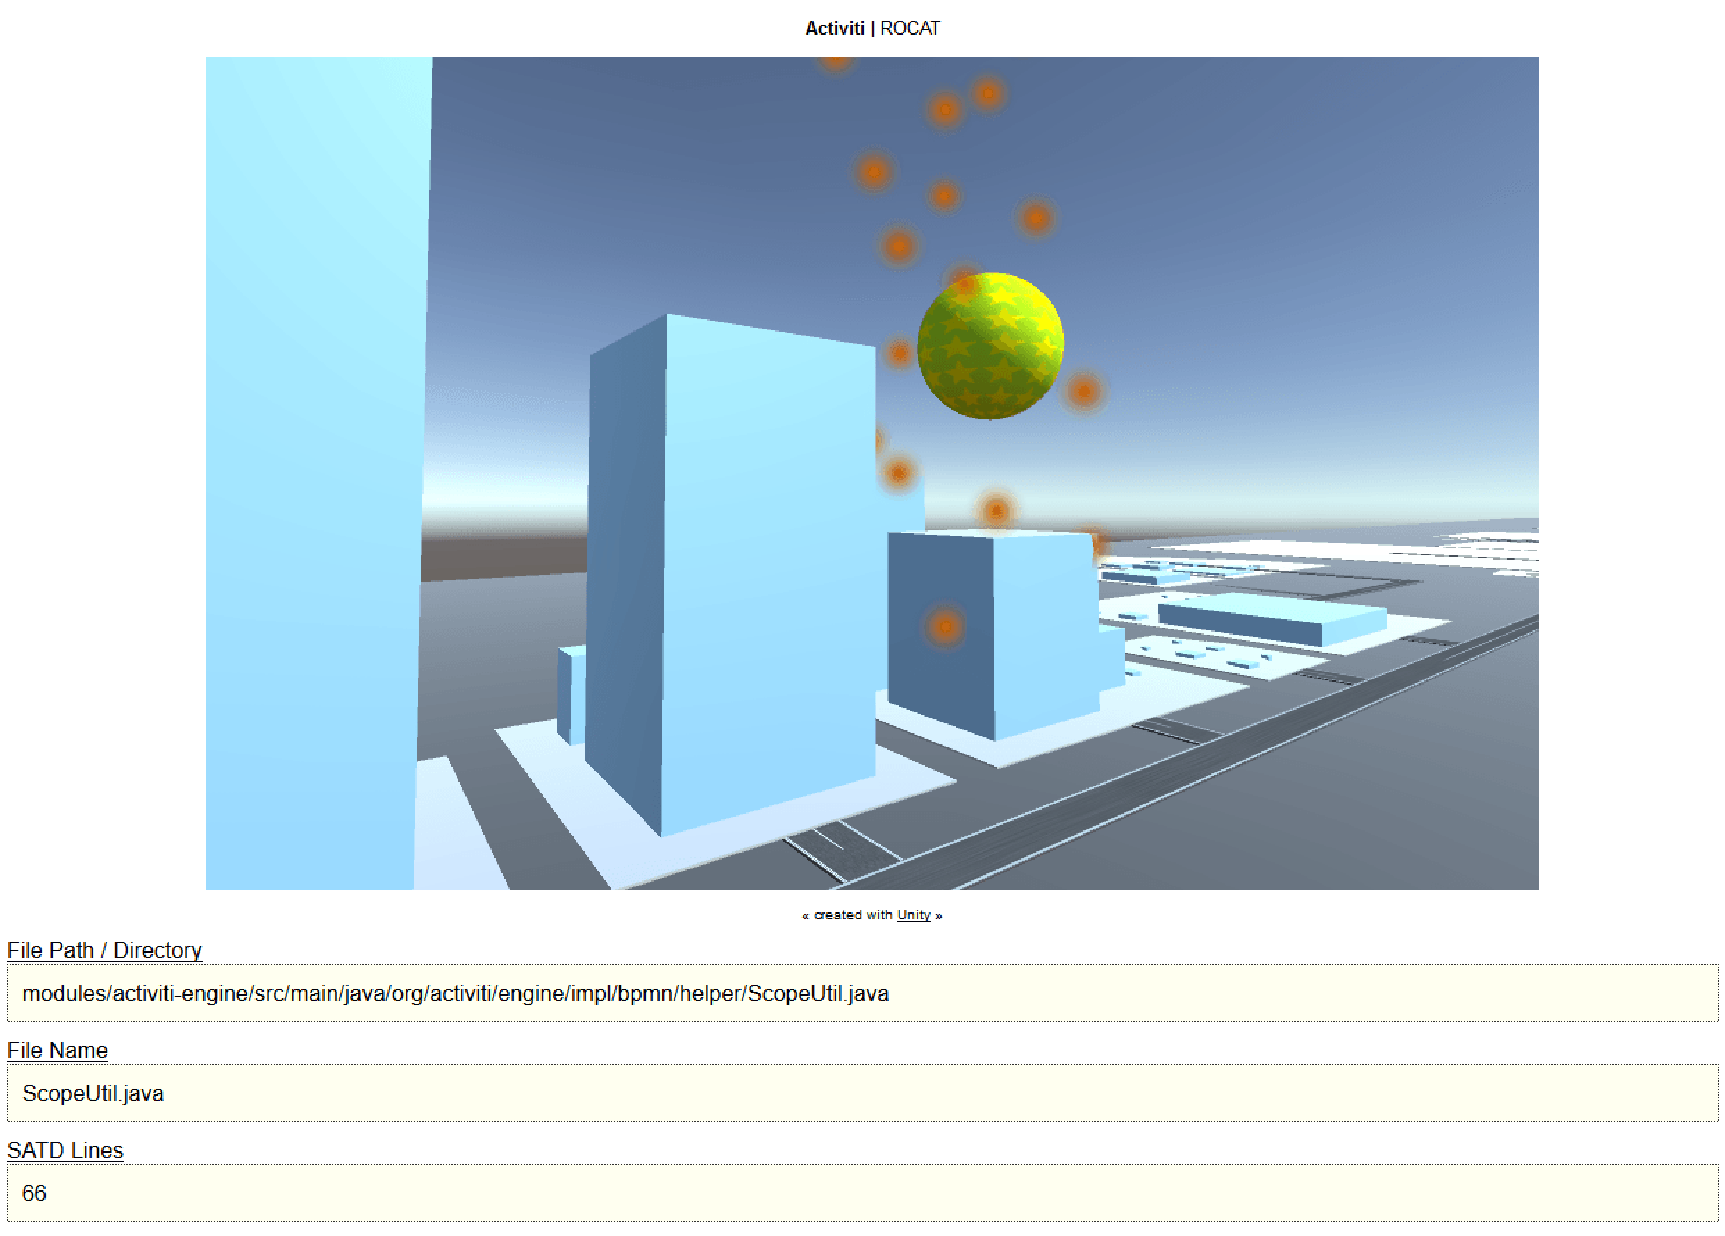
\includegraphics[width=\linewidth]{satd.pdf}
\caption{Visualization for self-admitted technical debt}
\label{figure:SATD}
\end{figure*}

\section{Discussions and Future Work}
We strongly believe that visualization is a crucial part of successful software engineering. 
Currently topics such as software analytics, team collaboration, learning/comprehension, and knowledge sharing are being studied separately, but we believe that a visual environment can be the center of these topics.

This paper presents a code city for multiple software development environments, named \textsf{Rocat}.
To develop this new visual software environment, we have also presented \textsf{Rocat} on \textsf{Kataribe} to provide software analytics for communities.

Now we are developing a system using \textsf{Rocat} that visualizes self-admitted technical debt (SATD). 
Technical debt is a metaphor that has been used to express non-optimal solutions of software development, and SATD is a kind of technical debt that is intentionally introduced into source code with keywords such as ``TODO'' or ``FIXME'' \cite{6976075}.
\figref{figure:SATD} shows a screen capture of the system.
The green ball and orange bubbles are markers of SATD.
The users can find files that contain SATD without reading source codes and share information about which files need refactoring.
We would like to evaluate our system with interviews with OSS developers, and then analyze their repositories to see the changes after introducing the system into development.

Furthermore, \textsf{Rocat} can visualize the relationship among source codes with program structures at the same time.
For example, in the case of call-graph visualization, 2D visualization can represent this relationship by using nodes and edges, but it is difficult to visualize other metrics clearly in the same view. 
\textsf{Rocat}, however, can visualize such a relationship with a bridge between buildings. 
Developers can understand a call graph and program structure at the same time.
This approach will be able to accelerate debugging tasks, for example.


\section*{Acknowledgments}
This work has been supported by JSPS KAKENHI Grant Number 16H05857 and the JSPS Program for Advancing Strategic International Networks to Accelerate the Circulation of Talented Researchers: Interdisciplinary Global Networks for Accelerating Theory and Practice in Software Ecosystem (G2603).
We would like to thank Yusuke Saito and Shin Fujiwara for their initial work on \textsf{Rocat}, and Takao Nakagawa and Stevche Radevski for their suggestions and advices.



\bibliographystyle{IEEEtran}
\bibliography{ref,reference-hata}

\end{document}
